\documentclass[a4paper,10pt]{article}
\usepackage[utf8]{inputenc}
\usepackage[utf8]{inputenc}
\usepackage[spanish]{babel}
\selectlanguage{spanish}
\usepackage{url}
\usepackage{graphicx}
\usepackage{float}

%opening
\title{Detección automática de flashes de impacto en videos planetarios}
\author{Joaquín Bogado}

\begin{document}

\maketitle

\begin{abstract}
Los flashes de impacto son fenómenos transitorios que pueden observarse en la superficie 
de gigantes gaseosos como Júpiter o Saturno o en la Luna (en la superficie no iluminada). 
Estos flashes se producen por la colisión o el ingreso a la atmósfera de asteroides de 
diferentes tamaños y pueden observarse con telescopios modestos y equipo al alcance de 
astrónomos amateur.

Este trabajo explica detalladamente el funcionamiento de una nueva técnica utilizada por 
astrónomos profesionales y observadores amateur para detectar posibles flashes de impacto 
en videos de observaciones planetarias, especialmente en videos de Júpiter y Saturno, de 
manera automática.

Como resultado de aplicar la técnica de Lucky Imaging, es común capturar varios 
minutos de video en los cuales es posible observar flashes de impacto. Sin embargo, es una 
tarea ardua revisar 40 minutos de video buscando eventos de entre 1 y 3 segundos de 
duración, más teniendo en cuenta que la mayoría de las sesiones de observación dicho 
evento no aparece. Es de vital importancia entonces realizar esta tarea utilizando 
software que procese los videos por lotes.

\end{abstract}

\section{Introducción}
En julio de 1994, los fragmentos del cometa Shoemaker-Levy 9 ingresaron a la atmósfera 
joviana y por primera vez en la historia, la humanidad estaba mirando. Si bien este 
evento, hasta ese momento, único permitió el estudio de capas de nubes normalmente 
ocultas a la vista de los astrónomos, también despertó interrogantes en la comunidad 
científica acerca de cuán frecuentes serían estos impactos.

Sin embargo, responder dicha pregunta, implica monitorear permanentemente a Júpiter y 
Saturno durante un período considerable de tiempo. Esto no es factible desde un solo 
observatorio (ya que solo se pueden realizar observaciones durante la noche) pero tampoco 
puede hacerse utilizando la red de observatorios internacionales, ya que los astrónomos 
deben dividirse el tiempo de utilización de estos observatorios entre los diversos 
proyectos de investigación. Fue así que los astrónomos profesionales recurrieron a la 
comunidad amateur.

Durante los años 90 y principios de 2000, los astrónomos amateur se vieron beneficiados 
por la reducción de costos de los sensores de captura digitales\cite{1} y por los 
importantes avances en las técnicas de captura y procesado de imágenes\cite{2}. El 
día de hoy, con relativamente poco dinero, es posible tomar fotografías del cielo 
nocturno con validez científica, desde el patio de nuestra casa. Mejor aún, los 
astrónomos amateur están repartidos alrededor del mundo en ambos hemisferios y pueden 
cubrir un rango de observación diario mayor que el de cualquier observatorio profesional 
que trabaje por su cuenta.

Esto se refleja en el número de producciones científicas que involucran a observadores 
amateur, el cual ha experimentado un importante aumento desde principios de 2000, como 
puede verse en la figura \ref{proam-plot}.

\begin{figure}[H]
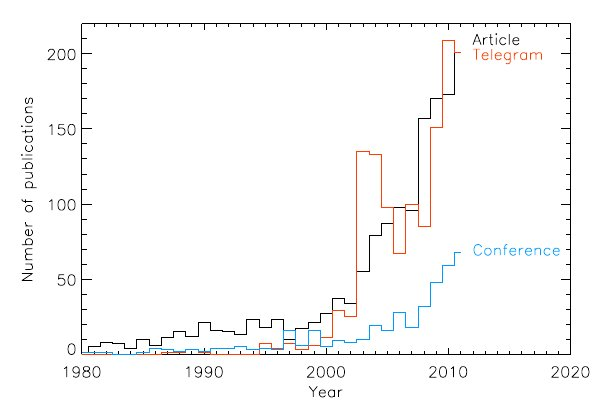
\includegraphics[scale=0.65]{proam-plot.jpg}
\caption{Estadísticas que muestran el incremento del número de publicaciones que 
involucran observadores amateur. Fuente: \cite{3}}
\label{proam-plot}
\end{figure}

Existen diversas asociaciones que hacen de nexo entre los observadores amateur y los 
profesionales. Entre ellas, la International Outer Planets Watch (IOPW) cuenta con una 
base de datos de observaciones, la gran mayoría realizadas por la comunidad amateur 
llamada Planetary Virtual Observatory and Laboratory 
(PVOL)\footnote{\url{http://www.pvol.ehu.es/pvol/}}.
Otras asociaciones como la Association of Lunar and Planetary Observers in 
Japan (ALPO-Japan)\footnote{http://alpo-j.asahikawa-med.ac.jp/indexE.htm}, la Société 
Astronomique de France (SAF)\footnote{http://www.astrosurf.com/saf/SAF} o la Association 
of Lunar and Planetary Observers (ALPO)\footnote{http://alpo-astronomy.org/ALPO}, no solo 
son frecuentadas por astrónomos profesionales en busca de las últimas observaciones 
realizadas por los amateur, sino que también brindan ayuda a los observadores nóveles y 
publican nuevas técnicas y software para mejorar la calidad científica de las 
observaciones amateur. Dichas asociaciones son de vital importancia en la colaboración 
PRO/AM.

\begin{figure}[H]
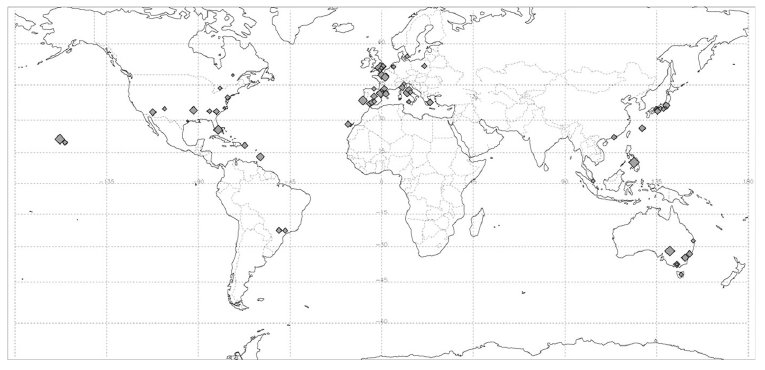
\includegraphics[scale=0.65]{amateur-map.jpg}
\caption{Localización geográfica de astrónomos amateur que reportan frecuentemente a la  
PVOL. Fuente: \cite{4}}
\label{amateur-map}
\end{figure}

\section{La técnica de Lucky Imaging}
Una técnica ampliamente difundida entre los observadores planetarios amateur es la que se 
denomina Lucky Imaging. Si bien los fundamentos de dicha técnica datan de 1978\cite{5}, 
no fue hasta que aparecieron las webcams que los astrónomos amateur comenzaron a 
experimentar con la obtención de imágenes de alta resolución utilizando esta técnica.

Dado que esta técnica aplicada a la obtención de imágenes de estrellas variables se 
explica con detalles en \cite{6} y con menor detalle pero aplicada a fotografía 
planetaria en \cite{1} y \cite{2}, solo se explicaran aquí y de manera somera solo los 
aspectos necesarios del funcionamiento de esta técnica necesarios para la aplicación del 
método descripto en este trabajo en la sección \ref{sec-core}.

El problema con la obtención de fotografías de alta resolución de la Luna o los planetas 
desde observatorios terrestres es que la atmósfera de la tierra produce distorsiones que 
degradan el rendimiento teórico de los equipos astronómicos. Estas distorsiones son 
transitorias y se producen como consecuencia de las diferentes densidades (debido a la 
temperatura) y direcciones (debido al viento) de las capas atmosféricas que la luz debe 
atravesar hasta llegar al sensor de la cámara.
Dado que este efecto es transitorio, existe una probabilidad mayor que cero de que en una 
secuencia de fotos, una en particular no esté distorsionada. Esta probabilidad depende, de 
acuerdo al trabajo de David Fried\cite{5}, del frame rate y del ángulo sólido de cielo que 
cubre el sistema sensor/telescopio. Básicamente, cuanto más grande dicho ángulo, es decir, 
cuanto mayor sea la porción de cielo que se desea fotografiar y cuanto más lento el frame 
rate, menor será la probabilidad de obtener una foto sin distorsión.

En fotografía planetaria, existen dos aspectos que hacen que esta técnica sea 
relativamente fácil de aplicar. Por un lado, los planetas como Júpiter o Saturno cubren 
un área de entre 30 y 60 segundos de arco (arc sec), a diferencia de la Luna o las 
fotografías de espacio profundo que cubren varios minutos de arco, es decir, la porción 
de cielo a fotografiar es pequeña. Por otra parte, a medida que el frame rate aumenta, 
se reduce la sensibilidad del sensor, con lo que los objetos más tenues no pueden ser 
fotografiados a un frame rate muy elevado. Sin embargo, Júpiter, Saturno, Venus, Mercurio 
y la Luna son objetos son relativamente brillantes, con lo que se pueden usar frame rates 
del orden de decenas a cientos. 

Entre los astrónomos amateur la técnica se aplica capturando un video al mayor frame rate 
posible de manera que el objeto a fotografiar tenga un histograma balanceado. La duración 
del video depende de varios aspectos pero por lo general no supera los 60 segundos 
duración en Júpiter ni 90 segundos en Saturno ya que la rotación de estos planetas se 
hace evidente a grandes aumentos y esta tiende a introducir blur en los detalles. Este 
video luego es procesado utilizando programas como Registax o Autostackert, los cuales 
seleccionan un porcentaje de los mejores frames de acuerdo a algún criterio (bordes más 
afilados, frecuencias más altas, Strehl ratio) y luego registran y apilan dichos frames 
(técnica de shift and add) y producen una única foto de mayor calidad y resolución que 
cualquiera de los frames individuales del video. Esta técnica se aplica utilizando cámaras 
color, pero los amateur más serios utilizan cámaras monocromáticas más filtros específicos 
para obtener información más detallada de la luz del objeto\footnote{Así lo explica 
Christoper Go en el video que puede verse en 
\url{https://www.youtube.com/watch?v=8MeZhlV7p_Y}. C. Go es uno de los más experimentados 
fotógrafos planetarios de la comunidad, y es autor de varios descubrimientos incluyendo la 
reaparición la Oval VA en 2006 y la reaparición del cinturón ecuatorial sur en 2010.}. 
Para obtener una fotografía en color utilizando una cámara monocromática, se debe repetir 
el procedimiento filmando un video con un filtro azul, otro con un filtro verde y otro con 
un filtro rojo. Además, suele tener importancia científica la luz reflejada en el 
infrarrojo cercano, para lo que es común utilizar un filtro long pass en las longitudes de 
onda 700-1000nm. 

Como resultado de aplicar la técnica de Lucky Imaging, es común terminar con varios 
minutos (por experiencias propias, entre 10 y 40 minutos) de video en los cuales es 
posible observar flashes de impacto. Sin embargo, es una tarea ardua revisar 40 minutos 
de video buscando eventos de entre 1 y 3 segundos de duración, más teniendo en cuenta que 
la mayoría de las sesiones dicho evento no aparece. Es de vital importancia entonces 
realizar esta tarea por software y de manera automática.
\section{Historia de los flashes de impacto}
Los primeros registros de flashes de impacto en Júpiter fueron registrados en 1994 
cuando los fragmentos de cometa Shoemaker-Levy 9 ingresaron a la atmósfera joviana. Dado 
que el impacto fue predicho con antelación, pudo ser registrado por diversos 
observatorios alrededor del mundo. En \cite{7} puede verse un gif donde se ve el flash de 
impacto producido por uno de los fragmentos. La captura es de uno de los observatorios 
Max Planck Insitute y está basada en capturas en la banda del infrarrojo. En \cite{8} y 
\cite{9} existe una colección de fotos mantenida por NASA con los registros del fenómeno 
realizado por diferentes instituciones.

En 2009, el programador y astrónomo amateur australiano Antony Wesley descubrió una marca 
de impacto en sus fotografías de Júpiter\cite{10}. El descubrimiento fue corroborado por 
fotografías del Telescopio Espacial Hubble, entre otros observatorios.

\begin{figure}[H]
\centering
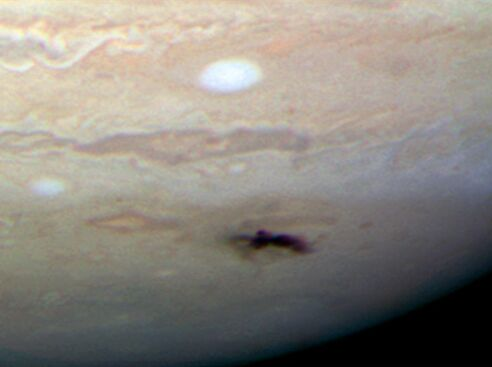
\includegraphics[scale=0.45]{Hs-2009-23-crop.jpg}
\caption{Imagen del Telescopio Espacial Hubble de la marca de impacto descubierta por A. 
Wesley en 2009. Imagen en dominio público.}
\label{amateur-map}
\end{figure}

Recién en junio de 2010 fue cuando se capturó un flash de impacto en video\cite{11}. El 
evento fue filmado simultáneamente por Antony Wesley desde Australia y Christoper Go 
desde Filipinas.  Previo a este descubrimiento, los científicos no sabían que este tipo 
de fenómenos podía observarse y abrió el interrogante de cuantos de estos se producían 
normalmente.
\begin{figure}[H]
\centering
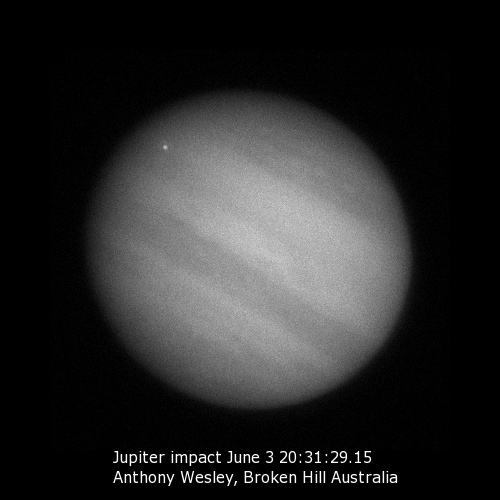
\includegraphics[scale=0.45]{wesley-2010.jpg}
\caption{Primer flash de impacto capturado en video. RAW Frame \copyright(A. Wesley, 
2010.)}
\label{amateur-map}
\end{figure}
En agosto de 2010, el amateur Masayuki Tachikawa de Japón observó un fenómeno similar en 
una de sus capturas\cite{12}. En septiembre de 2012 el astrónomo Dan Petersen observó y 
reporto un flash, que más tarde fue confirmado en video por George Hall, un astrónomo 
amateur de Estados Unidos. El evento filmado por Hall fue adquirido utilizando una webcam 
barata\cite{13}.

En marzo de 2016, un nuevo impacto fue registrado desde Austria por Gerrit Kernbauer, 
utilizando un telescopio de solamente 20 cm de apertura. Este evento más tarde fue 
confirmado por John McKeon, quien observaba desde Irlanda con un equipo un poco más 
importante\cite{14}

Ninguno de estos impactos dejó marcas en la superficie de Júpiter y no hubiera 
sido posible descubrirlos excepto por los registros en video de estos astrónomos 
aficionados.

\section{Algoritmo de identificación de flashes de impacto}
\label{sec-core}
Existen dos paquetes de software que implementan algoritmos de detección de flashes de 
impacto, ambos con un funcionamiento muy similar basado en la técnica de fotometría 
diferencial\cite{15}. Dado que el software DeTeCt\cite{16} presenta algunas mejoras 
respecto a JID\cite{17}\cite{18}, se estudiarán sus algoritmos como referencia para este 
trabajo. El método de detección utilizado por DeTeCt se explica en detalle en \cite{19}. 
DeTeCt utiliza dos algoritmos que se detallan a continuación:

Sea $$V = \{I_1, I_2, ... , I_n\}$$ una secuencia de imágenes. El primer paso consiste en 
registrar el video. El proceso de registro garantiza cada pixel $(x,y)$ del frame de 
referencia $I_r$ se corresponde con el mismo feature del objeto a fotografiar en todos 
los $I_n$ frames del video $V$. Esto se logra simplemente calculando el centro masa del 
planeta en el frame $I_x$ y haciendo un shift para que las coordenadas de este centro de 
masa se correspondan con la del frame de referencia, usualmente $I_1$.

\subsection{Detección basada en el diferencial de intensidad}
El primer algorimo trata de determinar un incremento temporal en el brillo de un pixel, 
evento asociado a la aparición de algún posible flash de impacto. Asumiendo que el 
brillo de un pixel no varía demasiado en el tiempo, podemos detectar un flash de 
impacto si detectamos un pixel que se aleje mucho de su brillo promedio.
Sea entonces $I_i(x,y)$ la intensidad del pixel de la posición $(x,y)$ en el frame $I_i$, 
decimos que un pixel es candidato a mostrar un flash de impacto cuando la diferencia 
entre el brillo medio y el máximo es mayor que cierto umbral $k$. Podemos decir que hay 
un candidato a flash de impacto en el frame $i$ si la intensidad de alguno de sus 
pixels $I_i(x,y)$ cumple que:
$$I_i(x,y) - \frac{1}{n}\sum_{i=1}^{n}I_i(x,y) \geq k$$
Cuan grande o chico es este umbral depende de la captura y en general es un parámetro que 
las herramientas permiten configurar a mano.

En la figura \ref{pixel-plot} puede verse el perfil de 4 pixels de un video de 500 frames 
filmado por A. Wesley\footnote{El video en cuestión puede descargarse desde el sitio 
\url{https://jupiter.samba.org/jupiter/20100603-203129-impact/red-3000-3500.avi}}. En el 
pixel $(115,97)$ del frame 189 puede apreciarse un flash de impacto. Los pixels 
inspeccionados pueden verse en la figura \ref{pixel-location}
\begin{figure}[H]
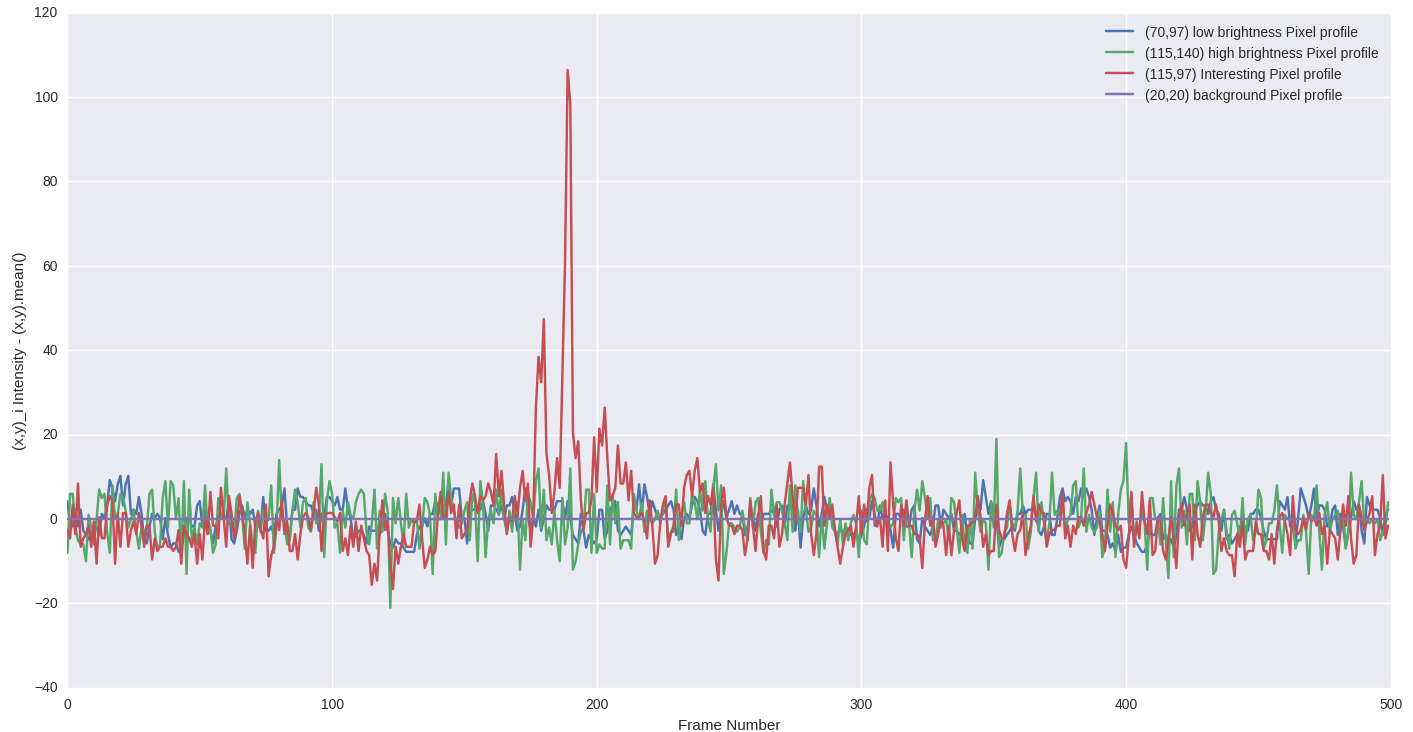
\includegraphics[scale=0.35]{pixprof2.png}
\caption{Diferencia entre la intensidad de un pixel y su media para los 500 frames para 
los pixesl (70,97), (115,40), (20,20) y (115,97) }
\label{pixel-plot}
\end{figure}
Para eliminar fluctuaciones en un pixel solo, tanto JID como DeTeCt realizan la búsqueda 
en una vecindad de $3x3$ de cada pixel. JID además permite configurar la vecindad de 
detección.

\subsection{Detección basada en inspección visual}
El problema del algoritmo anterior, es que por un lado genera falsos positivos y 
sobretodo falsos negativos, dependiendo de la selección del umbral. DeTeCt además genera 
por cada video, un juego de tres imágenes para su inspección visual.

La primera imagen muestra para cada pixel $(x,y)$, el promedio de los pixels $I_i(x,y), 
i= 1,...,n$.
$$I_{avg}(x,y) =  \frac{1}{n}\sum_{i=1}^{n}I_i(x,y)$$
La segunda imagen muestra para cada pixel $(x,y)$, el máximo de los pixels $I_i(x,y), 
i= 1,...,n$.
$$I_{max}(x,y) =  max(I_i(x,y)), i=1,...,n$$
La tercera imagen muestra la diferencia entre $I_{max}(x,y)$ y $I_{avg}(x,y)$.
$$I_{diff}(x,y) = I_{max}(x,y) - I_{avg}(x,y)$$
La figura \ref{detect} muestra un ejemplo de estas tres imágenes calculadas sobre el 
video de A. Wesley.

Estas imágenes pueden servir a los efectos de realizar una rápida inspección visual para 
determinar si los reportes de detección del software son falsos positivos o negativos.

\begin{figure}[H]
\centering
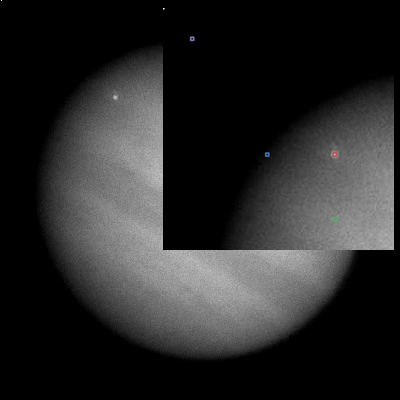
\includegraphics[scale=0.75]{red189.jpg}
\caption{Localización de los pixels (70,97), (115,40), (20,20) y (115,97) en el video de 
A. Wesley.}
\label{pixel-location}
\end{figure}

\begin{figure}[H]
\centering
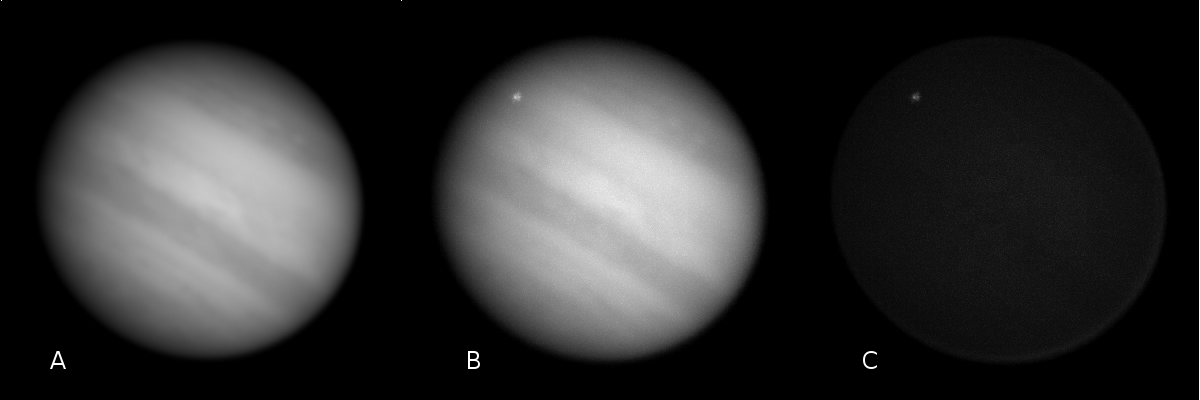
\includegraphics[scale=0.25]{detect.png}
\caption{A:$I_{avg}$, B: $I_{max}$ y C: $I_{diff}$}
\label{detect}
\end{figure}

\section{Conclusiones}
Se describen en este trabajo, dos técnicas nóveles para la detección de flashes de 
impacto en Júpiter, aunque las mismas técnicas son aplicables a videos de Saturno, las 
cuales han servido para estudiar la taza real de impactos en dichos planetas, si bien no 
para establecerlas a ciencia cierta, para poner cotas importantes\cite{20}.

El software de análisis con los que se generaron los gráficos de las sección 
\ref{sec-core} es de mi propia autoría y se provee para su evaluación adjunto a la 
entrega de este trabajo.

\begin{thebibliography}{99}
\bibitem{1} \url{
http://www.cloudynights.com/page/articles/cat/articles/astrophotography/ccd-cameras-and-di
gital-cameras/digital-astrophotography-beginners-guide-r127}
\bibitem{2} \url{
http://www.ast.cam.ac.uk/research/instrumentation.surveys.and.projects/lucky.imaging/lates
t.results/amateur.lucky.imaging}
\bibitem{3} Diversos autores. PRO-AM collaborations in Planetary Astronomy. Vol. 8, 
EPSC2013-197, 2013.
\bibitem{4} Diversos autores. Instrumental methods for professional and amateur 
collaborations in planetary astronomy. Springer. 2014.
\bibitem{5} D. L. Fried. Probability of getting a lucky short-exposure image through 
turbulence. Journal of the Optical Society of America Vol. 68, Issue 12, pp. 1651-1658. 
1978
\bibitem{6} Nicholas Michael Law. Lucky Imaging: Diffraction - Limited Astronomy From The 
Ground In The Visible. Thesis disertation. Cambridge, 2006.
\bibitem{7}Impacto de uno de los fragmentos de SL9. \url{
https://en.wikipedia.org/wiki/File:Max_Planck_Institute_Shoemaker%E2%80%93Levy_9.gif}. 
Imagen de dominio público.
\bibitem{8}Archivo fotográfico de NASA. SL9 Impact.
\url{http://nssdc.gsfc.nasa.gov/planetary/sl9/comet_images.html}
\bibitem{9}\url{http://nssdc.gsfc.nasa.gov/planetary/sl9/html/sl9whatsnew.html}
\bibitem{10}\url{https://jupiter.samba.org/jupiter-impact.html}
\bibitem{11}\url{http://www.nasa.gov/topics/solarsystem/features/jupiter20100909.html}
\bibitem{12}\url{http://cosmicdiary.org/fmarchis/2010/08/22/another-flash-on-jupiter/}
\bibitem{13}\url{http://cosmicdiary.org/fmarchis/2012/09/10/another-fireball-on-jupiter/}
\bibitem{14}\url{
http://www.slate.com/blogs/bad_astronomy/2016/03/29/jupiter_hit_by_asteroid_or_comet_in_ma
rch_2016.html}
\bibitem{15} Michael Richmond. Differential Photometry. \url{
http://spiff.rit.edu/classes/phys373/lectures/diff_photom/diff_photom.html}. 
Licencia Creative Commons by-nc-sa 2.0.
\bibitem{16}\url{http://www.astrosurf.com/planetessaf/doc/dtc/doc/dtc_tuto_en.htm}
\bibitem{17}J. C. Moreno. Manual de Jupiter Impact Detection Software. Programa Para La 
Detección De Impactos En Júpiter. 2012.
\bibitem{18}JID home page. \url{http://www.astrosurf.com/jcmoreno/proyectos/jid/jid.htm}
\bibitem{19} M. Delcroix, R. Hueso. Jovian impact flashes detection with DeTeCt software 
project. EPSC2013-812. 2013.
\bibitem{20} Projet de détection de flash d'impacts avec le logiciel DeTeCt.
\url{http://www.astrosurf.com/planetessaf/doc/project_detect.shtml}
\end{thebibliography}


\end{document}
